\documentclass[12pt,letterpaper,titlepage]{article}

\usepackage{fontspec}
\defaultfontfeatures{Mapping=tex-text}
\usepackage{xunicode}
\usepackage{xltxtra}
\usepackage{amsmath}
\usepackage{pdfpages}
\usepackage{amsfonts}
\usepackage{bbold}
\usepackage{amssymb}
\setcounter{secnumdepth}{0}
\usepackage{nameref}
\usepackage{enumitem}
\usepackage{environ}
\usepackage{pgfplots}
\usepackage{listings}

\showboxdepth=\maxdimen
\showboxbreadth=\maxdimen


\usepackage{paracol}
\usepackage{wrapfig}
\globalcounter{table}
\globalcounter{figure}
\usepackage{graphicx}
\usepackage[left=1in,right=1in,top=1in,bottom=1in]{geometry}
\graphicspath{{img/}}

\author{Jacob Abel}
\title{	Design \& Simulate 12
	\\\large ECE2204 CRN:82929
}

\setlength{\parskip}{0.5em}

\begin{document}
\maketitle
\begin{raggedright}

\section{Problem 12.3-4.a.1: } Adapted ePMOS to eNMOS and changed values.
\subsection{Design}

Calculate the drain current and drain-to-source voltage of a common source circuit with a n-channel enhancement-mode MOSFET. Assume $R_1 = 50k\Omega$, $R_2 = 100k\Omega$, $R_D = 10k\Omega$, $V_{DD} = 5V$, $V_TN = 1V$, and $K_N = 0.03 mA/V^2$.

\begin{center}
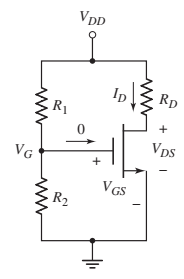
\includegraphics[width=\textwidth, height=12\baselineskip, keepaspectratio=true]{ds1}
\end{center}

\begin{align*}
   V_G = V_{GS}
     &= \frac{R_2}{R_1 + R_2}(V_{DD})
      = \frac{100k\Omega}{150k\Omega}(5V)
      = 3.\overline{3}V
\\ I_D
	 &= K_N(V_{GS} - V_{TN})^2
	  = (0.03mA/V^2)(3.\overline{3}V - 1V)^2
	  = 0.163mA
\\ V_{DS}
	 &= V_{DD} - I_DR_D
	  = 5V - 0.163mA \times 10k\Omega
	  = 3.37V
\\ V_{DS}(\text{sat})
	 &= V_{GS} - V_{TN}
	  = 3.\overline{3}V - 1V
	  = 2.\overline{3}V
\end{align*}

$V_{DS} > V_{DS}(\text{sat})$ and therefore the transistor is in the saturation region. 

The drain to source voltage is $V_{DS} = 3.37V$ and the drain current is $I_D = 0.163mA$.

\clearpage
\subsection{Validation}

\begin{center}
LTSpice Implementation (values within $<1\%$)
\columnratio{0.5}
\begin{paracol}{2}
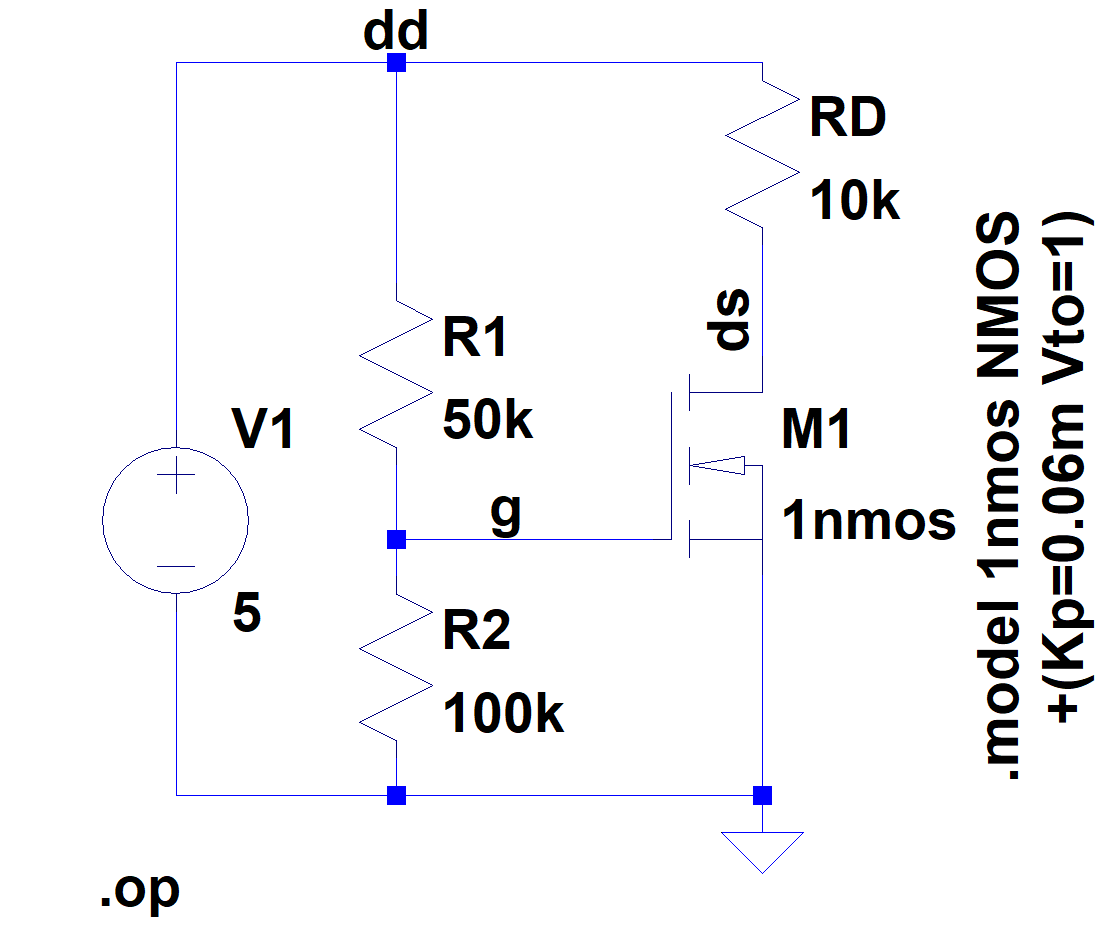
\includegraphics[width=.48\textwidth, height=\textheight, keepaspectratio=true]{ds1b}
\switchcolumn
\begin{tabular}{|l|l|c|}
  \hline V(dd):	& 5	            & voltage
\\\hline V(g):	& 3.33333	    & voltage
\\\hline V(ds):	& 3.36667	    & voltage
\\\hline Id(M1):& 0.000163333	& device\_current
\\\hline Ig(M1):& 0	            & device\_current
\\\hline Ib(M1):& -3.37667e-012	& device\_current
\\\hline Is(M1):& -0.000163333	& device\_current
\\\hline I(Rd):	& 0.000163333	& device\_current
\\\hline I(R2):	& 3.33333e-005	& device\_current
\\\hline I(R1):	& 3.33333e-005	& device\_current
\\\hline I(V1):	& -0.000196667	& device\_current
\\\hline
\end{tabular}
\end{paracol}
$Err_{V_{DS}} = \frac{|3.37-3.36667|}{3.37} = 0.000988 = 0.09\%$

$Err_{I_D} = \frac{|163-163.333|}{163} = 0.00204 = 0.20\%$
\end{center}

\clearpage
\section{Problem 12.3-4.b.1: } Adapted from Problem 3.26 on page 197 by changing some values, switching eNMOS to ePMOS.
\subsection{Design}

Considering the circuit below, assume that the transistor is instead an ePMOS, $R_S$ and $R_D$ are swapped, $V_{TP} = 0.75V$, $K_p = 0.25 mA/V^2$, and $V_{DD} = 12V$. Calculate $V_{SG}$, $I_D$, and $V_{SD}$.

\begin{center}
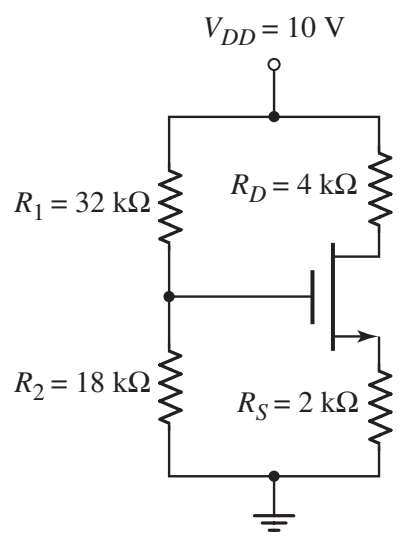
\includegraphics[width=\textwidth, height=12\baselineskip, keepaspectratio=true]{ds2}
\end{center}

\begin{align*}
   V_G
     &= \frac{R_2}{R_1 + R_2}(V_DD)
      = \frac{18k\Omega}{32k\Omega+18k\Omega}(12V)
      = 4.32V
\\ V_{SG}
     &= V_{DD} - V_G
      = 12V - 4.32V
      = 7.68V
\\ I(R_1) &=
\\ I(R_2)
	 &= \frac{V_{DD} - V_G}{R_1}
	  = \frac{12V - 7.68V}{32k\Omega}
	  = 0.24mA
\end{align*}

\clearpage
\begin{align*}
  & V_{DD} - I_D (R_S + R_D) = V_{SG} + V_T
\\\implies& V_{DD} - K_P(V_{SG}+V_T)^2 (R_S + R_D) = V_{SG} + V_T
\\\implies& 12V - (0.25 mA/V^2)(V_{SG} - 0.75V)^2 (2k\Omega + 4k\Omega) = V_{SG} - 0.75V
\\\implies& V_{SG} = 3.264V
\end{align*}

\begin{align*}
    V_{SD}
  	  &= V_{SG} + V_T
  	   = 3.264V - 0.75V
  	   = 2.514V
\\  I_D
      &= K_P(V_{SG} + V_T)^2
       = (0.25 mA/V^2)(3.264V-0.75V)^2
       = 1.58mA
\end{align*}



\subsection{Validation}

\begin{center}
LTSpice Implementation (values within $<1\%$)
\columnratio{0.52}
\begin{paracol}{2}
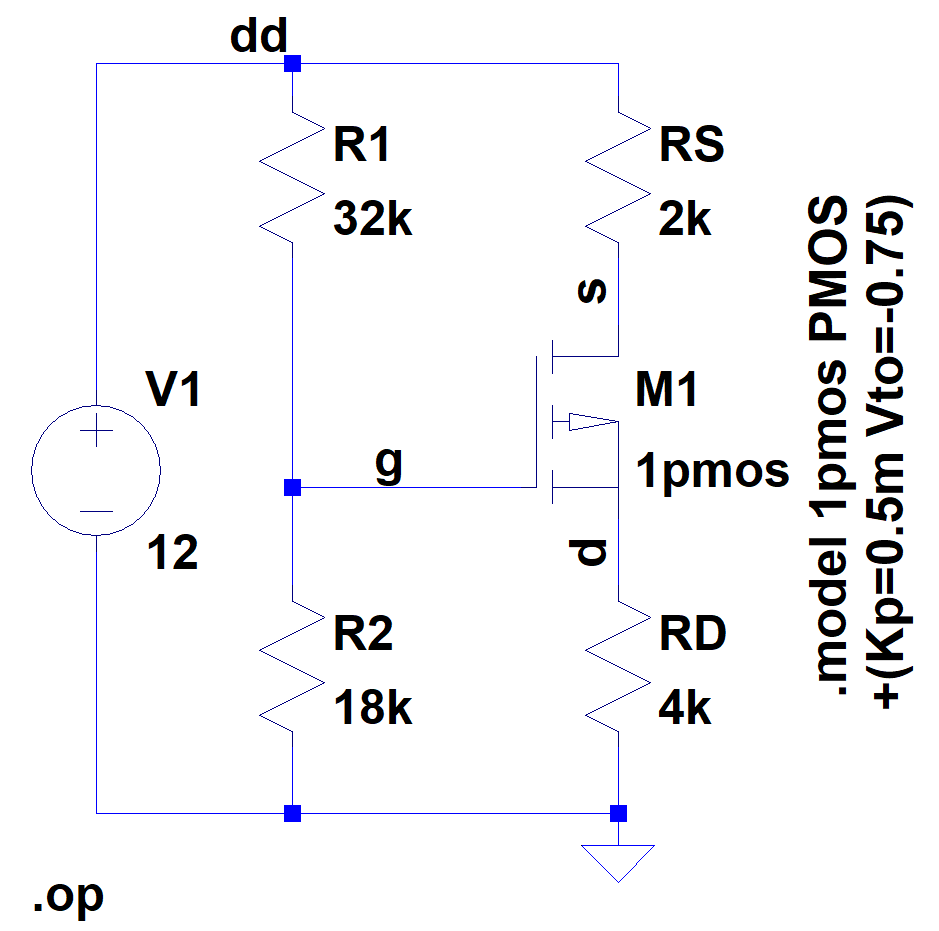
\includegraphics[width=.5\textwidth, height=\textheight, keepaspectratio=true]{ds2b}
\switchcolumn
\begin{tabular}{|l|l|c|}
  \hline V(dd):	& 12        	& voltage
\\\hline V(g):	& 4.32  	    & voltage
\\\hline V(s):	& 8.2186    	& voltage
\\\hline V(d):	& 7.56279   	& voltage
\\\hline Id(M1):& 0.00195211	& device\_current
\\\hline Ig(M1):& -0        	& device\_current
\\\hline Ib(M1):& -0.00102718	& device\_current
\\\hline Is(M1):& -0.000924925	& device\_current
\\\hline I(Rd):	& 0.0018907	    & device\_current
\\\hline I(Rs):	& 0.0018907	    & device\_current
\\\hline I(R2):	& 0.00024	    & device\_current
\\\hline I(R1):	& 0.00024	    & device\_current
\\\hline I(V1):	& -0.0021307	& device\_current
\\\hline
\end{tabular}
\end{paracol}
\end{center}

Note to grader: This problem gave me a lot of trouble. I know the results deviate from the simulation. If you could leave a note explaining where I messed up, that would be greatly appreciated.


This assignment should demonstrate a basic understanding of MOSFET transistor circuits.

\textit{I have neither given nor received unauthorized assistance on this assignment.}


\end{raggedright}
\end{document}
